\section{Evaluation}
\label{sec:Evaluation}
In this section we show different experiments that were run on the different approaches and analyse their running times, as well as the number of iterations in the inner most loop or their recursive calls respectively.
First, we give an overview over different grammars, that were used, and explain how we expect the algorithms to behave when parsing input strings on them.
All of them are in (reduced) Chomsky Normal Form.

\subsection{Grammars}
\subsubsection{Dyck Language}
This language consists of all words, that have the correct amount of opening and closing parentheses, i.e., strings of the form '()...()' or '((...))'.
The grammar that builds these words has the rules:
\begin{align*}
    S&\rightarrow SS|LA|LR\\
    A&\rightarrow SR\\
    L&\rightarrow (\\
    R&\rightarrow )\\
\end{align*}

We will run experiments on words of the language, as well as on strings with additional single parentheses, i.e., ')()...()' and ''()...()(', which are not part of the language.

For this grammar, we expect top-down to run faster on strings of the form '()..()'.
The algorithm iterates over the rules in the order as they were parse to the program, thus $S\rightarrow SS$ is the first rule.
It then iterates over different splitting points, starting with $k=1$, which will not find a solution, as $S$ can not yield any of the substrings, since they have a different amount f opening and closing parentheses.
when trying $k=2$, \texttt{Top-Down($S$, $1$, $2$)} is called, which will return true.
For the right hand side of the string, this will be repeated.
Thus, with the first rule of the grammar and the second splitting point, the optimal answer is returned and the algorithm is expected to terminate relatively fast.

For strings of the form '((..))', the top-down algorithm will look at a lot more subproblems while looking for the solution.
Different from strings of the form '()..()' this string has no partitioning into two substrings, where $S$ can yield both substrings.
All rules have to be applied on $S$ at least once, thus a lot more rules and parts of the string will be considered before the answer is found.

Further, ')()..()' is parsed faster than '()..()(' by the top-down algorithm.
The way the algorithm was implemented makes us not look at the right part of a splitting (second call of \texttt{Top-Down} on line 10 in algorithm\ref{alg:td}).
This means, when the first symbol in the string violates the constraints of the language, we look at the left hand side of every partitioning, find that it can not be yielded, and terminate.
If, on the other hand, the last symbol violates the constraint, we will find for a lot of splitting points, that $S$ can yield the left substring, and check the right substring.
This yields in a lot more subproblems which have to be considered, and thus in a longer running time.


\subsubsection{Strings Starting or Ending in a}
This grammar contains all worlds with an arbitrary number of a's and b's in any order, but starting resp. ending with a.
The rules for strings starting with a are:
\begin{align*}
    S&\rightarrow AB\\
    B&\rightarrow BB|a|b\\
    A&\rightarrow a\\
\end{align*}

and those for strings ending in a:
\begin{align*}
    S&\rightarrow BA\\
    B&\rightarrow BB|a|b\\
    A&\rightarrow a\\
\end{align*}

For both of these grammars we will run tests on strings of the form 'ab..ab' and 'ba..ba'.
We expect a similar behavior as in the Dyck grammar.
The bottom-up approach will take a similar amount of time for both sets of test strings with either grammar.
Top-down on the other hand will perform better on the strings that are in the language for both grammars, as well as when parsing the strings not starting in a with the grammar starting in a.
It performs worse when parsing strings that do not end in a with the grammar that ends in a, with the same reasoning as we applied for the Dyck language.
Top down runs faster, when the symbol that violates the constraint of the grammar is in the beginning of the string.


\subsubsection{Equal Numbers}
Equal numbers is a grammar, that yields all strings with the same amount of a's and b's.
This is achieved with the following rules:
\begin{align*}
    S&\rightarrow SS|AB|BA\\
    B&\rightarrow SB|BS|b\\
    A&\rightarrow a\\
\end{align*}

For this grammar we will test strings of the form aa..bb and ab..ab, as well as both of these sets with additional a's.
We expect both parser to run slower on this, than on strings starting with a.
It may be similar to strings ending in a though, since we always must look at the whole string.
An additional a in the end may be worse than one at the beginning.
It is also worse than parentheses on '()..()', but similar to '((..))'.
top-down will be faster on ab..ab than bottom up.
\todo{think more about expectations, very little time invested so far}

\subsubsection{A Finite Language}
\todo{come up with a finite language ?}

\subsection{Experiments}
We will now show the results of experiments, using the grammars described, and analyze whether  the algorithms behave as we expect them to behave.
In order to get better results, for each input string the parser was run 10 times.
The time showed in the plots is the average of the resulting running times, where the fastest and slowest times were excluded.

\subsubsection{Dyck Language}

\begin{figure}[!ht]
    \centering
    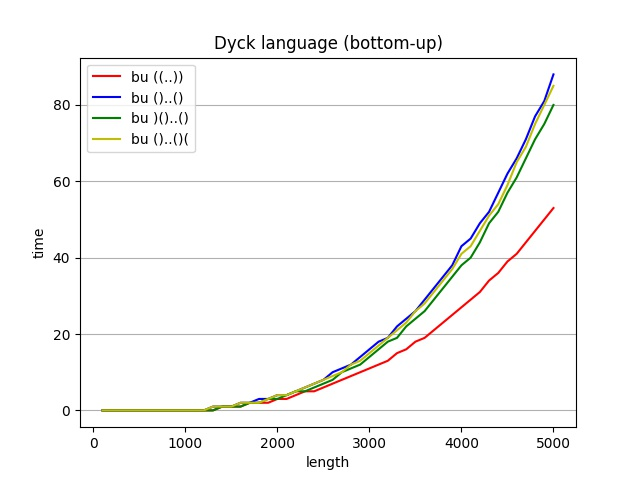
\includegraphics[width=0.6\textwidth]{Images/t_dyck_bu.jpg}
    \caption{Running time (s) of the bottom-up algorithm when parsing different set of strings of sizes 100-5000, in steps of hundred, for the Dyck Language.}
    \label{fig:t_dyck_bu}
\end{figure}

Figure~\ref{fig:t_dyck_bu} shows the running times of the bottom-up parser on different sets of input strings.
The strings were of length 100 to 5000, growing in steps of 100.
As we assumed, the times are very similar for all four different sets of input strings.
Parsing the strings of the form '((..))' is a little faster.
We do not know why.

The curves are asymptotically to $O(n^3)$, in fact, the yellow, blue and green line are very close to $6.4*10^{-10}*n^3$.

We split the parsings of top-down into two plots.
The first one, Figure~\ref{fig:t_dyck_td_slow}, is for the slow cases, where we did not run the parser on strings longer than 2500
The second one, Figure~\ref{fig:t_dyck_td_fast}, was for the fast cases, where we extended the test set to contain strings up to a size of 10000.

\begin{figure}[h!]
    \centering
    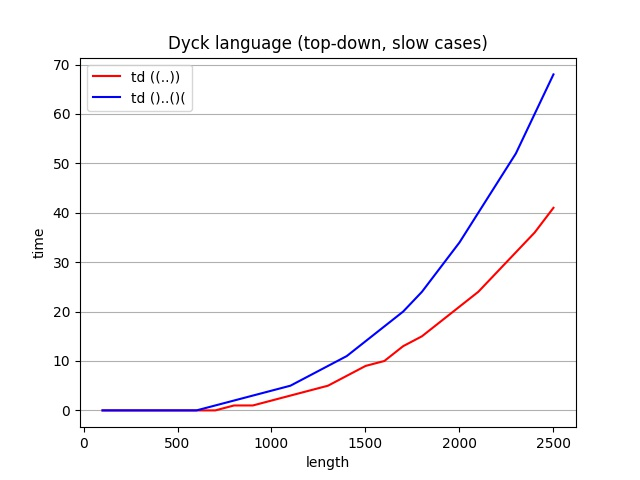
\includegraphics[width=0.6\textwidth]{Images/t_dyck_td_slow.jpg}
    \caption{Running time (s) of the top-down algorithm when parsing two set of strings of sizes 100-2500, in steps of hundred, for the Dyck Language.}
    \label{fig:t_dyck_td_slow}
\end{figure}

\begin{figure}[h!]
    \centering
    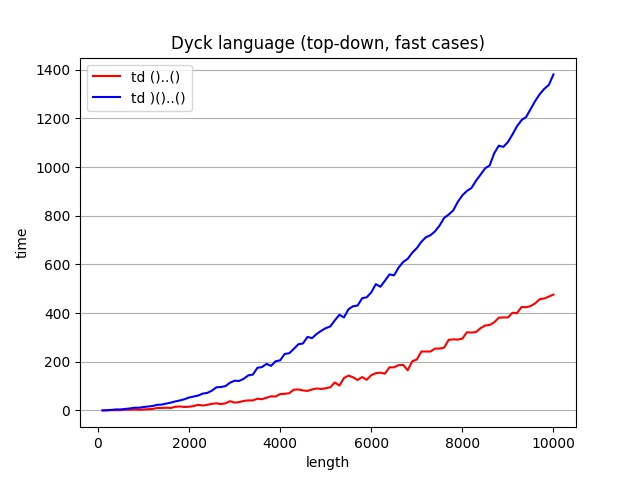
\includegraphics[width=0.6\textwidth]{Images/t_dyck_td_fast.jpg}
    \caption{Running time (ms) of the top-down algorithm when parsing two set of strings of sizes 100-10000, in steps of hundred, for the Dyck Language.}
    \label{fig:t_dyck_td_fast}
\end{figure}

As we assumed, parsing the test sets of strings of the form '((..))' and '()..()(' with top-down was a lot slower than parsing the strings of the other two sets.
While parsing strings of the form '()..()(' of length 2500 took almost 70 seconds, parsing strings of the form '()..()' of length 10'000 took only 0.4 seconds.

The fast cases are a lot faster than the bottom-up parser.
This is the case, because bottom up fills all cells of $tab$, regardless of whether or not they are needed to find the solution, while top down only fills the one needed to find the optimal solution.
When the rules of the grammar are in a favorable order and the splitting points for finding subproblems that yield the optimal solution is low, as it is the case in the fast cases of Dyck, it can be very fast.

However, if this is not the case, then the parser may take a lot of time.
We can see this at the slow cases of the Dyck language.
Here, the parser behaves a lot worse than bottom up.
This may be due to the fact, that bottom up fills the cells of $tab$ in a structured way, accessing the already filled cells of $tab$ not more often, then needed to fill the other cells.
Top-down on the other hand may run into the same subproblems very often.
This means the algorithm calls itself recursively and to access the cell of the same subproblem more often than bottom up does.
Since recursive calls are more time consuming, and more accesses may be performed, this results in a potentially very bad running time.

\begin{figure}[h!]
    \centering
    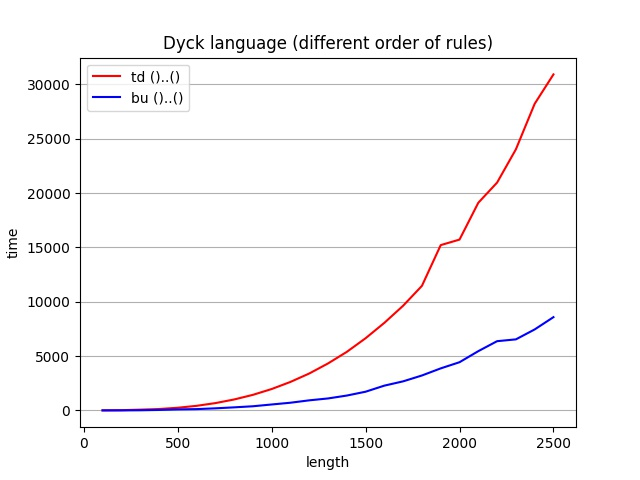
\includegraphics[width=0.6\textwidth]{Images/t_dyck_order.jpg}
    \caption{Running time (ms) of both algorithms for parsing a set of strings of sizes 100-2500, in steps of hundred, for the Dyck Language, with a different order of the rules.}
    \label{fig:t_dyck_order}
\end{figure}

I order to verify the hypothesis, that the order of rules matters for the top-down parser, we run experiments on the same grammar, but with the rules of $S$ in opposite order.
The results can be seen in figure~\ref{fig:t_dyck_order}.
The parser is in fact a lot slower than it was before, thus the order of the rules may play a major rule, when parsing.
We further see that it does not matter that much for the bottom up parser.
It has almost the same running time, than it had with the original ordering of the rules.

\subsection{Strings starting and ending in a}

The running times achieved, did not meat the expectations.
Surprisingly, both the top down and bottom-up algorithm performed very differently on the two grammars, being very fast at parsing for the grammar for words starting in a, and slower for words ending in a.
In general, we see that the times are lower than they were for the Dyck language.
This is presumably because this grammar has only two non-terminal rules, which leads to less subproblems which have to be considered.

We split the results in three graphs, one for the running times of both parsers on the grammar ending in a (Figure~\ref{fig:t_ea_td_bu}), one for top-down and one for bottom-up, each for the grammar starting in a (Figure~\ref{fig:t_sa_td} and ~\ref{fig:t_sa_bu} respectively).

\begin{figure}[h!]
    \centering
    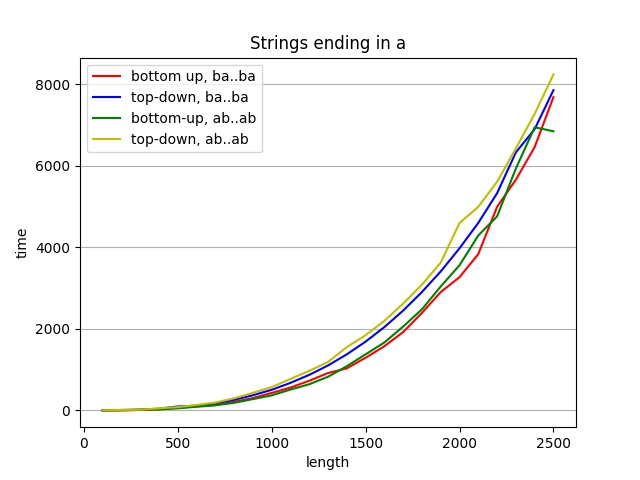
\includegraphics[width=0.6\textwidth]{Images/t_ea_td_bu.jpg}
    \caption{Running time (ms) of the bottom-up and top-down algorithm when parsing two set of strings of sizes 100-2500, in steps of hundred, for the Language of words ending in a.}
    \label{fig:t_ea_td_bu}
\end{figure}

We see, that the curves for parsing the grammar ending in a are almost identical with the ones of the bottom up parser run on the Dyck Language.

\begin{figure}[h!]
    \centering
    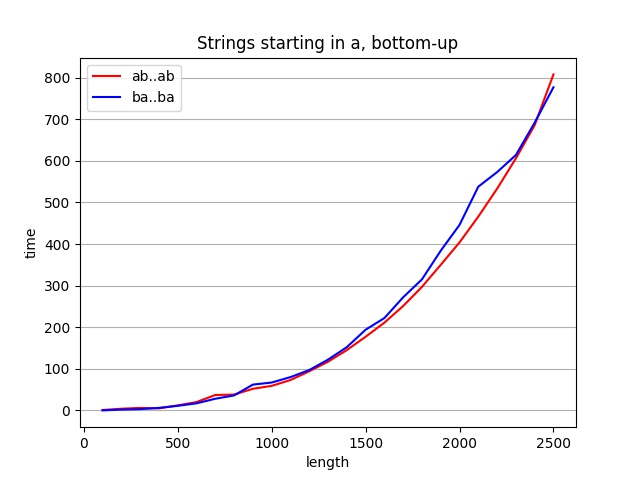
\includegraphics[width=0.6\textwidth]{Images/t_sa_bu.jpg}
    \caption{Running time (ms) of the bottom-up algorithm when parsing two set of strings of sizes 100-2500, in steps of hundred, for the Language of words starting in a.}
    \label{fig:t_sa_bu}
\end{figure}

However, the running times for the grammar for strings starting in a are a lot faster.
If we consider how $tab$ will be filled by the algorithm, it becomes clear, why that is.
Remember that $tab$ for this grammar is $3\times n\times n$, since it has three non-terminal variables.
we will look at the two dimensional table of each non-terminal.

The table for $A$, say $tab_A$, has true only in the row for substrings of length 1 and where the symbol is $a$.
As it has no non-terminal rule, when trying to fill the reminder of $tab_A$ the algorithm proceeds very fast, since no splitting has to be considered, as the corresponding loop over $k$ is never even accessed.

The table for $B$, $tab_B$, has true in all cells.
All substrings of length one can be yielded, since $B$ has the two terminal rules $B\rightarrow a|b$.
Further, since its only non-terminal rule is $B\rightarrow BB$, when trying to fill a new cell of $tab_B$, only other cells of $tab_B$ must be considered.
BEcause they are all true, the loop over the splitting point $k$ gets breaked after the first splitting point, thus filling $tab_B$ can be done in a slow matter, too.

Let's now look at $tab_S$.
Since the only rule for $S$ is $S\rightarrow AB$, first the cell of $tab_A$ gets accessed.
The first splitting point always generates a substring of length one, on the left of k.
If this is an a, then the corresponding cell in $tab_A$ is true, and we must access $tab_B-$ as well.
As we argued before, this value will always be true, we are thus not looking at any other splitting points.
If the substring is b, then the cell in $tab_A$ is false, and we will not look at $tab_B$, but continue to the next splitting point.

For the grammar for all words ending in a, $tab_A$ and $tab_B$ are filled in a very similar manner.
However, when filling $tab_S$ we have almost twice the amount of table accesses to $tab_B$.
Since the rule for $S$ is $S\rightarrow BA$, for every splitting point first $tab_B$ gets accessed, which will always return true, and then $tab_A$ gets accessed, which will return false in most cases.
Thus, both $tab_B$ and $tab_A$ are accessed for every $k$, while for strings starting in a $tab_B$ was only accessed when $tab_A$ was true.

For strings starting in a, we expect very similar running times for strings of the form aa..bb.
For strings ending in a, we expect worse running times for those strings.
We would expect it to be even worse for strings of the form ab..bb, while for strings starting in a it would result in a similar running time.
\todo{run experiments, include plots}


\begin{figure}[h!]
    \centering
    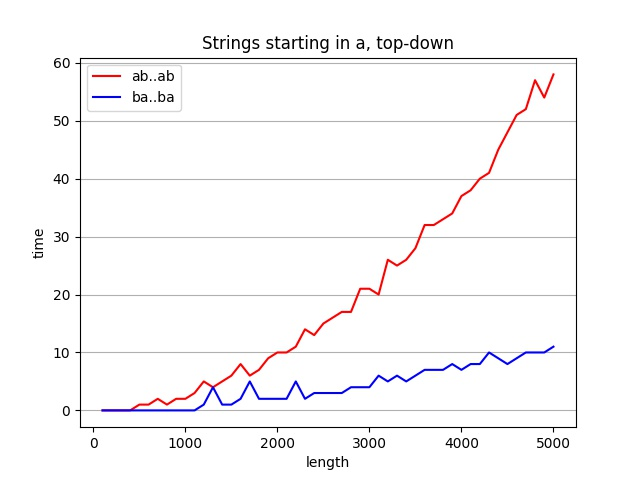
\includegraphics[width=0.6\textwidth]{Images/t_sa_td.jpg}
    \caption{Running time (ms) of the top-down algorithm when parsing two set of strings of sizes 100-5000, in steps of hundred, for the Language of words starting in a.}
    \label{fig:t_sa_td}
\end{figure}

as we see in Figure~\ref{fig:t_sa_td}, the running times for top-down were incredibly low.
The three bumps in the blue line are supposedly due to rounding errors of the compiler, seen as the times there are lower than 5 milliseconds.
The bumps appear on the red line at the same time after the same period of time after starting the parsers (not at the same length!), though not as distinctive as in the blue line, since the running times are already a little higher at this point.

The incredibly low running times can be explained with similar reasoning, as for the low running times of bottom up on strings starting with a.
Top down is even faster, since it does not fill $tab$ completely.
In fact, when parsing strings not starting in a for the grammar of strings starting in a, it will only ever look at the most left children of the recursive tree, since everything returns falls
This results in a ver low amount of recursive calls.
In fact, the number of calls on the recursive function is $\Theta(n)$ (figure~\ref{fig:c_sa_td}).
As we argued in section~\ref{sec:top_down}, the upper bound for this number is $O(n^3)$.
The numbers for the counter of bottom up (repetitions of the inner most loop, i.e. over splitting points k) for parsing strings for the grammar of strings starting in a, are somewhere in the middle of $n^2$ and $n^2$, still yielding relatively fast running times.

\begin{figure}[h!]
    \centering
    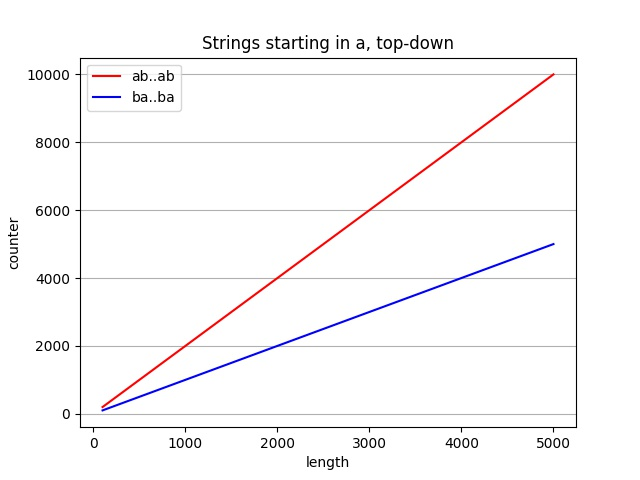
\includegraphics[width=0.6\textwidth]{Images/c_sa_td.jpg}
    \caption{Running time (ms) of the top-down algorithm when parsing two set of strings of sizes 100-5000, in steps of hundred, for the Language of words starting in a.}
    \label{fig:c_sa_td}
\end{figure}

\todo{Add subsection for evaluations of step 3}



